\chapter{Conclusion}\label{c:conclusion}


\section{Research Summary and Synthesis}

As we approach the conclusion of this dissertation, I would like to summarise the work undertaken throughout this research. This recap serves to articulate how the various threads of practice-based research, experiments, user studies, and conceptual frameworks have converged to address the core research questions and aims.

\subsection{Motivations and Aims}

I began by establishing that the emerging capabilities of AI systems increasingly warrant ascribing creative behaviour to them (for the full argument, refer to the introduction). This recognition opened the pressing question of how these systems might interact with and influence human creativity. While acknowledging that new technologies have historically interacted with, expanded, and affected human creativity in complex ways, I argued that AI presents a unique possibility: that of co-creativity. This perspective framed my core research aim:

\textit{Exploring how to design generative AI systems that act as effective co-creators, maintaining human involvement and agency while effectively leveraging the potential of this technology.}

I positioned this primarily as an interaction design problem—one that entails enabling modes of interaction that maintain human involvement and agency such that co-creativity can be realised. The potential for modelling dialogic interaction emerged as a design paradigm that could enable iterative back-and-forth engagement, facilitating mutual understanding of intentions, worldviews, and goals, as well as influence and interaction both through and about the creation itself.

This approach built upon the work of the larger Australian Research Council funded project on Dialogic Creative AI that I am part of, and drew from a rich literature that conceptualises human-AI interaction as a form of dialogue involving both language and non-language-based interactive dynamics. These considerations led to the formulation of three research questions:

\begin{quote}
\textbf{Research Questions:}

\begin{enumerate}
    \item \textit{R1: What is the potential of modelling dialogue in interaction design to enable effective human–AI co-creativity?}
    \item \textit{R2: What roles can humans and AI assume in co-creative processes, and in what ways can generative AI function as a co-creator?}
    \item \textit{R3: Which design principles can guide the development of co-creative systems?}
\end{enumerate}

\end{quote}

\subsection{Foundations: Dialogic Co-creativity}

The research began with the development of an early framework for dialogic interaction, presented in a paper at the 2022 CHI workshop on generative AI. At that time, language models functioned primarily as autocomplete systems, and I conducted an experiment exploring their potential to engage in back-and-forth dialogue. The results demonstrated that these systems were capable of bidirectional communication—switching within a single conversation between discussing at a meta-level (addressing goals, clarifications, and feedback) and contributing directly to the writing process.

While the quality of writing produced was limited, the experiment showed promise for a generative model that could act as a co-creator capable of engaging both at a meta-level and through the writing itself. In that paper, I proposed an early framework for dialogic co-creativity that identified a set of actions constituting dialogic interaction, categorized according to whether they operated through or about the creation.

Notably, this work was performed shortly before the rapid widespread adoption of large language models that interacted via dialogue,  which ocurred after the launch of ChatGPT in late 2022.

\subsection{Early Experiments: Narrative Device}

Continuing to explore the potential of large language models, in early 2022, I developed an experimental online tool called Narrative Device. This simple interface allowed users to input two words and receive a short story that combined these concepts. The intention was to test the potential of generative AI as a co-creative tool \textit{in the wild}.

The response was overwhelming—more than 2 million stories were generated, and hundreds of thousands of people used the tool. My server crashed multiple times due to overloads. I incurred in a substantial bill for AI model usage--north of 5k AUD--entirely funded from donations by users. This enthusiasm provided evidence to the potential of generative AI experiences that engaged both human creativity (in this case conceiving interesting word combinations) and AI creativity (in weaving these concepts into narratives). It also confirmed the potential of combinatorial creativity in machines as discussed by Boden \cite{Boden2003-hk}.

\subsection{The landscape changes: machines can communicate}

My previous experiments were conducted in a landscape where language models, and generative AI in general, remained largely unknown to the general population. However, almost a year after my Narrative Device experiment, this radically changed. ChatGPT was launched in late 2022, and soon it became rapidly adopted by millions of people, followed by the launch of similar chat-based AI competitors. This sudden change, which largely kickstarted the positionng if AI as a mainstream technology, provided me with three key insights:

\begin{enumerate}
    \item First, provided evidence to the potential of bidirectional communication that I had discussed in my first experiment and paper. As ChatGPT's creators acknowledged, and which I discuss in more detail in Chapter 1 and 3, the widespread adoption of ChatGPT was not due to an innovation at the model level (which was the same GPT-3.5 I had used for Narrative Device almost a year prior), but rather in this new mode of interaction in a conversational, dialogue-based format.
    \item People began using chat-based LLMs across a wide range of co-creativ tasks, primarily in writing domains. However, I observed that chat interfaces imposed limitations on effective co-creation in writing contexts. Users lacked a shared space to make direct contributions to text, being restricted to a sequence of messages. Editing required copying text to a separate editor, making changes, and then returning it to the chat interface for further iteration, imposing considerable friction for co-creation.
\end{enumerate}

\subsection{Beyond Chat: Collaborative Editing Interfaces}

Drawing from my conception of dialogic co-creativity, I noted that chat interfaces allowed users to interact \textit{about} the creation but not \textit{through} the creation itself. This arrangement, I hypothesised, led users to become less involved—making requests to the model rather than actively participating in the writing process.

Given my research aim of creating an interaction model where both humans and AI are deeply involved, I further hypothesised that an interface enabling both chat interaction and collaborative writing in a shared text editor would lead to greater human involvement. I implemented a prototype across two versions: a rudimentary first version where the model had to rewrite the entire text to make a single edit, and a more robust second version that allowed the model to make targeted edits using a schema I defined.

I conducted two studies to test these hypotheses:

\begin{enumerate}
    \item A controlled experiment comparing a chat-only interface with my prototype. Users of the chat-only interface more frequently reported that the AI did most of the work, while users of the editor interface were more likely to have contributed words to the final piece and described their roles as more involved and active.
    \item An in-depth qualitative study of users engaging with the hybrid chat + collaborative editor interface. Participants reported greater involvement compared to chat-only interfaces and described using the model to improve or polish their own writing rather than delegating the entire writing task. They also identified challenges related to understanding the editor, version control, and distinguishing between AI and human contributions.
\end{enumerate}

These studies demonstrated the potential of separating interaction through and about the creation, as well as the value of shared collaborative spaces beyond the now-dominant chat paradigm. However, they also highlighted the challenges in creating collaborative interfaces. Importantly, they also enriched my understanding of dialogic co-creativity as encompassing more than a mere two-way communication channel—it also required a shared collaborative space with it's own interaction dynamics.

\subsection{New Media Installations: Transformational Creativity}

Concurrent with my exploration of collaborative writing interfaces, I developed a creative practice in new media installations that investigated the potential of large language models in a different context. Rather than focusing on how these models could enhance established creative practices (enabling combinational or exploratory creativity in Boden's terms), I sought to explore their potential to create entirely new creative practices with their own sets of rules—what Boden would call transformational creativity.

I developed two installations that used language models to enable a new type of generative experience capable of acting and reacting within a context—interpreting environmental data and driving the continuous generation of audiovisual content. These works, developed in collaboration with my supervisor and Sydney-based music studio Uncanny Valley, were:

\begin{enumerate}
    \item \textbf{Systsem of a Sound}: Exhibited at the Australian National University
    \item \textbf{Music of the Sails}: Exhibited at the Sydney Opera House
\end{enumerate}

Both installations explored a novel role for AI collaboration that does not fit within existing paradigms—a role that a human could not play, which involved interpreting complex data and, as a result, continuously driving an audiovisual performance over multiple days, without stop. They also investigated the concept of \textbf{co-creating within and in response to a complex context encompassing social, economic, ecological, and built dimensions.}

While successfully realised, these projects also revealed limitations and challenges unique to AI systems. The black-box nature and \textbf{low explainability} of the models made \textbf{steering} them difficult, particularly given the generative artworks spanned multiple days of continuous generation. The LLM often fixated on certain outputs and choices, producing undesired content. It also highlighted the importance of maintaining rich histories of past interactions to enable the model to iterate and adjust based on previous outcomes and human guidance—forming a cycle of \textbf{mutual understanding and influence} with the human creator distributed across time.

\subsection{Visual Domains: Interior Design and Media}

On a concurrent thread, I explored the co-creative potential of generative AI in the visual domain, particularly design and media. 

\subsubsection{Interior Design Collaboration: Tilly}

Working with a Sydney-based interior design studio who reached out to me for collaboration, I developed Tilly in response to their specific request to create a design co-creator—an AI collaborator that would work alongside their team in their day-to-day practice. To fulfill this vision, I designed Tilly as a combination of language and image models accessible through a chat interface. The studio engaged with Tilly to ideate and generate designs for five innovative objects to be presented at Milan Design Week, combining elements of playfulness, sustainability, and wellbeing with novel materials.

Tilly proved most useful in \textbf{divergent} stages (ideation and generating multiple visual concepts) but showed limitations in \textbf{convergent} stages. Due to constraints of the image model, it struggled to \textbf{refine} and \textbf{iterate} on designs or explore preferred directions further, always generating new designs even with minor prompt adjustments.

Despite these limitations--or because of them--we sought to leverage the system's strengths in unique ways. Five visual concepts were generated and presented at Milan Design Week alongside tablets where visitors could interact with Tilly and provide feedback. Tilly then summarised this feedback and sent insights to the designers in Sydney, who used it to iterate on the designs over multiple rounds throughout the event. A few months later, the resulting designs were physically produced by artisans worldwide and exhibited at the London Design Festival.

Similar to the new media installations, this case study suggested that while AI may struggle with certain creative roles and tasks, particularly at convergent stages, it can assume novel roles that humans cannot—such as collecting and synthesising feedback from hundreds of people in parallel. This enabled a new form of distributed collective iterative co-creativity across time and space, involving designers, audience members, and the AI system itself.

\subsubsection{Visual Media: Australian Financial Review}

Lastly, in a case study with the Australian Financial Review, we explored using generative AI to create portraits for individuals featured in their annual Power List magazine. The publication wanted to generate portraits that would be \textbf{impossible} to capture with conventional photography—images that could tell a story about each individual's personality and work (e.g., the Head of the Federal Reserve piloting a hot air balloon as a metaphor for her control of inflation). Additionally, they aimed to spark discussion about the risks of deepfakes for high-profile individuals.

This case study involved training models for each person and navigating a fragmented workflow across various tools. We encountered similar limitations regarding \textbf{iteration}—sometimes generating images they liked but being unable to refine specific aspects without generating entirely new images. We also faced challenges around \textbf{control and consistency} in aligning with the publication's brand style and aesthetic, which we addressed by developing a hybrid workflow that combined multiple generative tools, manual post-processing techniques, and extensive output curation.

Ultimately, the images were printed in the magazine, including the cover and interior pages, and distributed nationally. As a research output, I published a paper outlining how the challenges of \textbf{iteration}, \textbf{control}, and \textbf{consistency} remain crucial limitations for effective human-AI co-creativity in visual domains.

\subsection{Evolved Understanding and Outcomes}

Throughout these diverse studies and explorations, my understanding of dialogic co-creativity evolved while maintaining its central importance as an analytical lens. Based on this evolved understanding, I revisited my framework established in Chapter 3, drawing from literature on dialogue across various disciplines to more precisely define dialogic interaction through six key elements:

\begin{enumerate}
    \item Bidirectional Communication
    \item A shared collaborative space
    \item Iteration
    \item Mutual Influence
    \item Mutual Understanding
    \item Contextual Awareness
\end{enumerate}

A figure graphically outlining this recapitulation of work is presented in Figure \ref{fig:recap}.

\begin{figure}
    \centering
    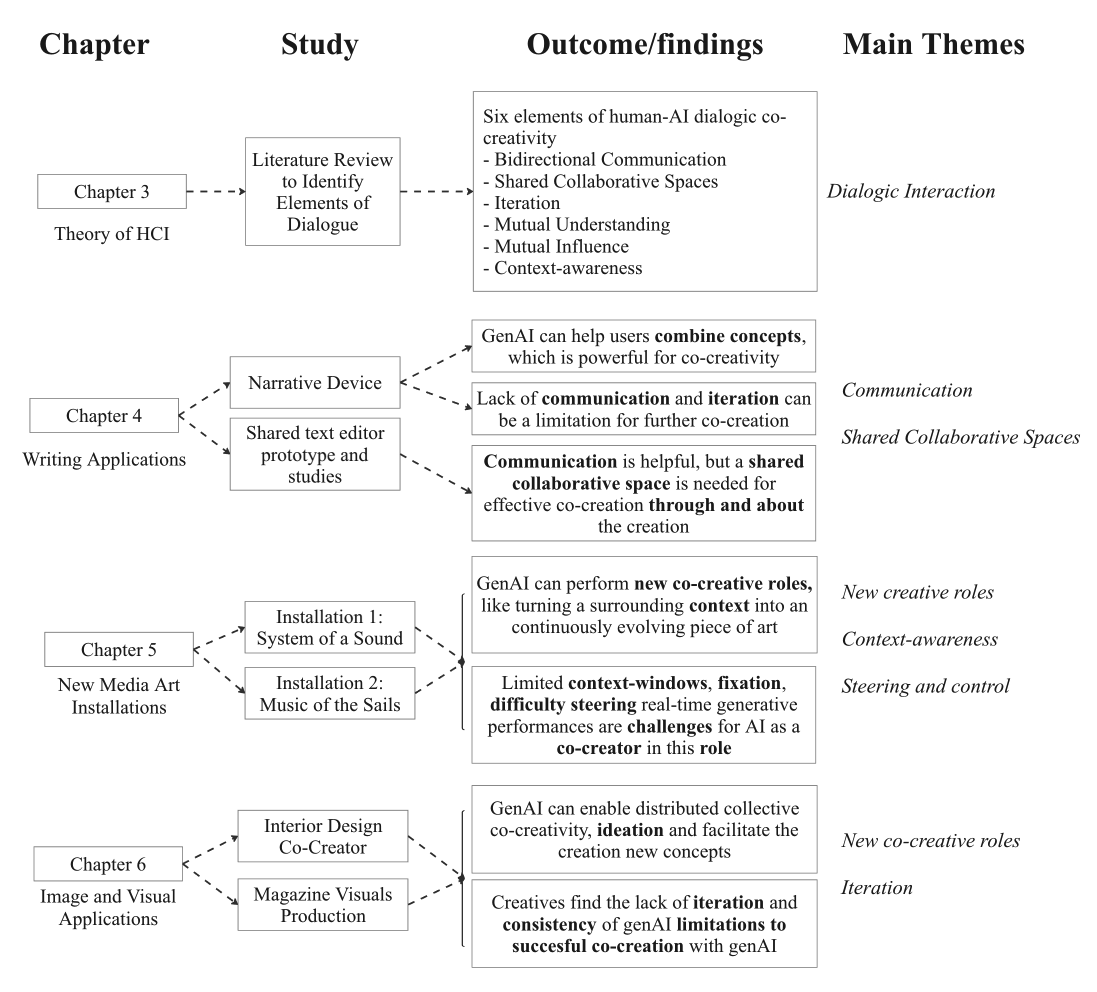
\includegraphics[width=1\linewidth]{chapteroutcomes.png}
    \caption{Diagram showing the outcomes and main themes from each chapter}
    \label{fig:recap}
\end{figure}

Now, in this concluding chapter, I distill this body of work into three key actionable outcomes that address my core research aim and each of my research questions:

\begin{enumerate}
    \item \textbf{Six Dimensions of Human-AI Co-creativity}: A framework of dimensions that designers and developers must consider when creating co-creative AI systems.
    \item \textbf{A Framework for Role Classification}: A systematic approach to classifying the roles that humans and AI can assume in co-creative processes.
    \item \textbf{Design Principles for Effective Co-creative AI}: A set of principles addressing each dimension and the roles humans and AI play in co-creative contexts.
\end{enumerate}

These outcomes provide practical guidance for the development of effective co-creative AI systems that maintain human involvement and agency while leveraging the unique capabilities of generative AI technologies.

\section{Six Dimensions of Human-AI Co-Creativity}

In recent years, multiple frameworks for guiding and characterising human-AI co-creativity have emerged. Early on \cite{Lubart2005-zi}, provided an initial characterisation of how humans and machines can partner in creative processes. More recently, Kantosalo (2020) introduced a three-layer framework that differentiates between interaction modalities—the sensory channels and devices for information exchange, interaction styles—the structural and behavioural patterns of collaboration (ranging from ambient to request-based and operation-based models), and interaction strategies—the evaluative metrics, goals, and meta-reasoning processes that underpin creative decision-making. In a similar vein, \cite{Rezwana2022-gg} proposed the COFI framework, which focuses on modelling interactions within human–AI co-creative systems by dividing the process into interactions between collaborators and with the artifact itself. More recently, in 2024, \cite{Moruzzi2024-cq} introduced a user-centered framework that outlines key dimensions of human–AI co-creativity. This framework enables users to modulate factors such as interaction, communication style, and level of expertise to adjust the degree of control in co-creative interactions. \cite{Llano2022-ti} developed a framework for explainable computational creative systems, outlining four principles: shared mental models, long-term memory, argumentation and exposing the creative process.

Similarly, \cite{Muller2020-nv} formulated an analytical framework for mixed-initiative generative AI applications that examines how agency and control are distributed between human and AI actors across different stages of the creative process.

This work builds upon and extends these existing frameworks whilst offering a distinct perspective on human-AI co-creativity. Unlike previous approaches that often emphasise technological capabilities or interaction taxonomies, this framework specifically addresses the design and development dimensions required for effective co-creative systems, particulary those that I explored throughout my thesis.

Central to my approach is the conceptualisation of co-creativity as fundamentally dialogic in nature. By drawing from the elements of dialogic interaction established in Chapter 3, I have constructed a framework that translates these principles into six concrete dimensions for system design. 

Although these dimensions are presented as distinct, they often overlap, and each facet may connect with aspects of another. They may change over time, and new ones may be added as the technology and our understanding of co-creativity develops. Therefore, I invite researchers to engage with these dimensions as such. It is my hope that this contribution to the growing field of human-AI co-creativity fosters dialogue and discussion. 

As such, the particular application of my six dimensions can be synthesised as follows: 

\begin{quote}
A robust co-creative AI system will be robust across the Six Dimensions of Human-AI Co-Creativity. 
\end{quote}

\subsection{The Six Dimensions}

\begin{figure}
    \centering
    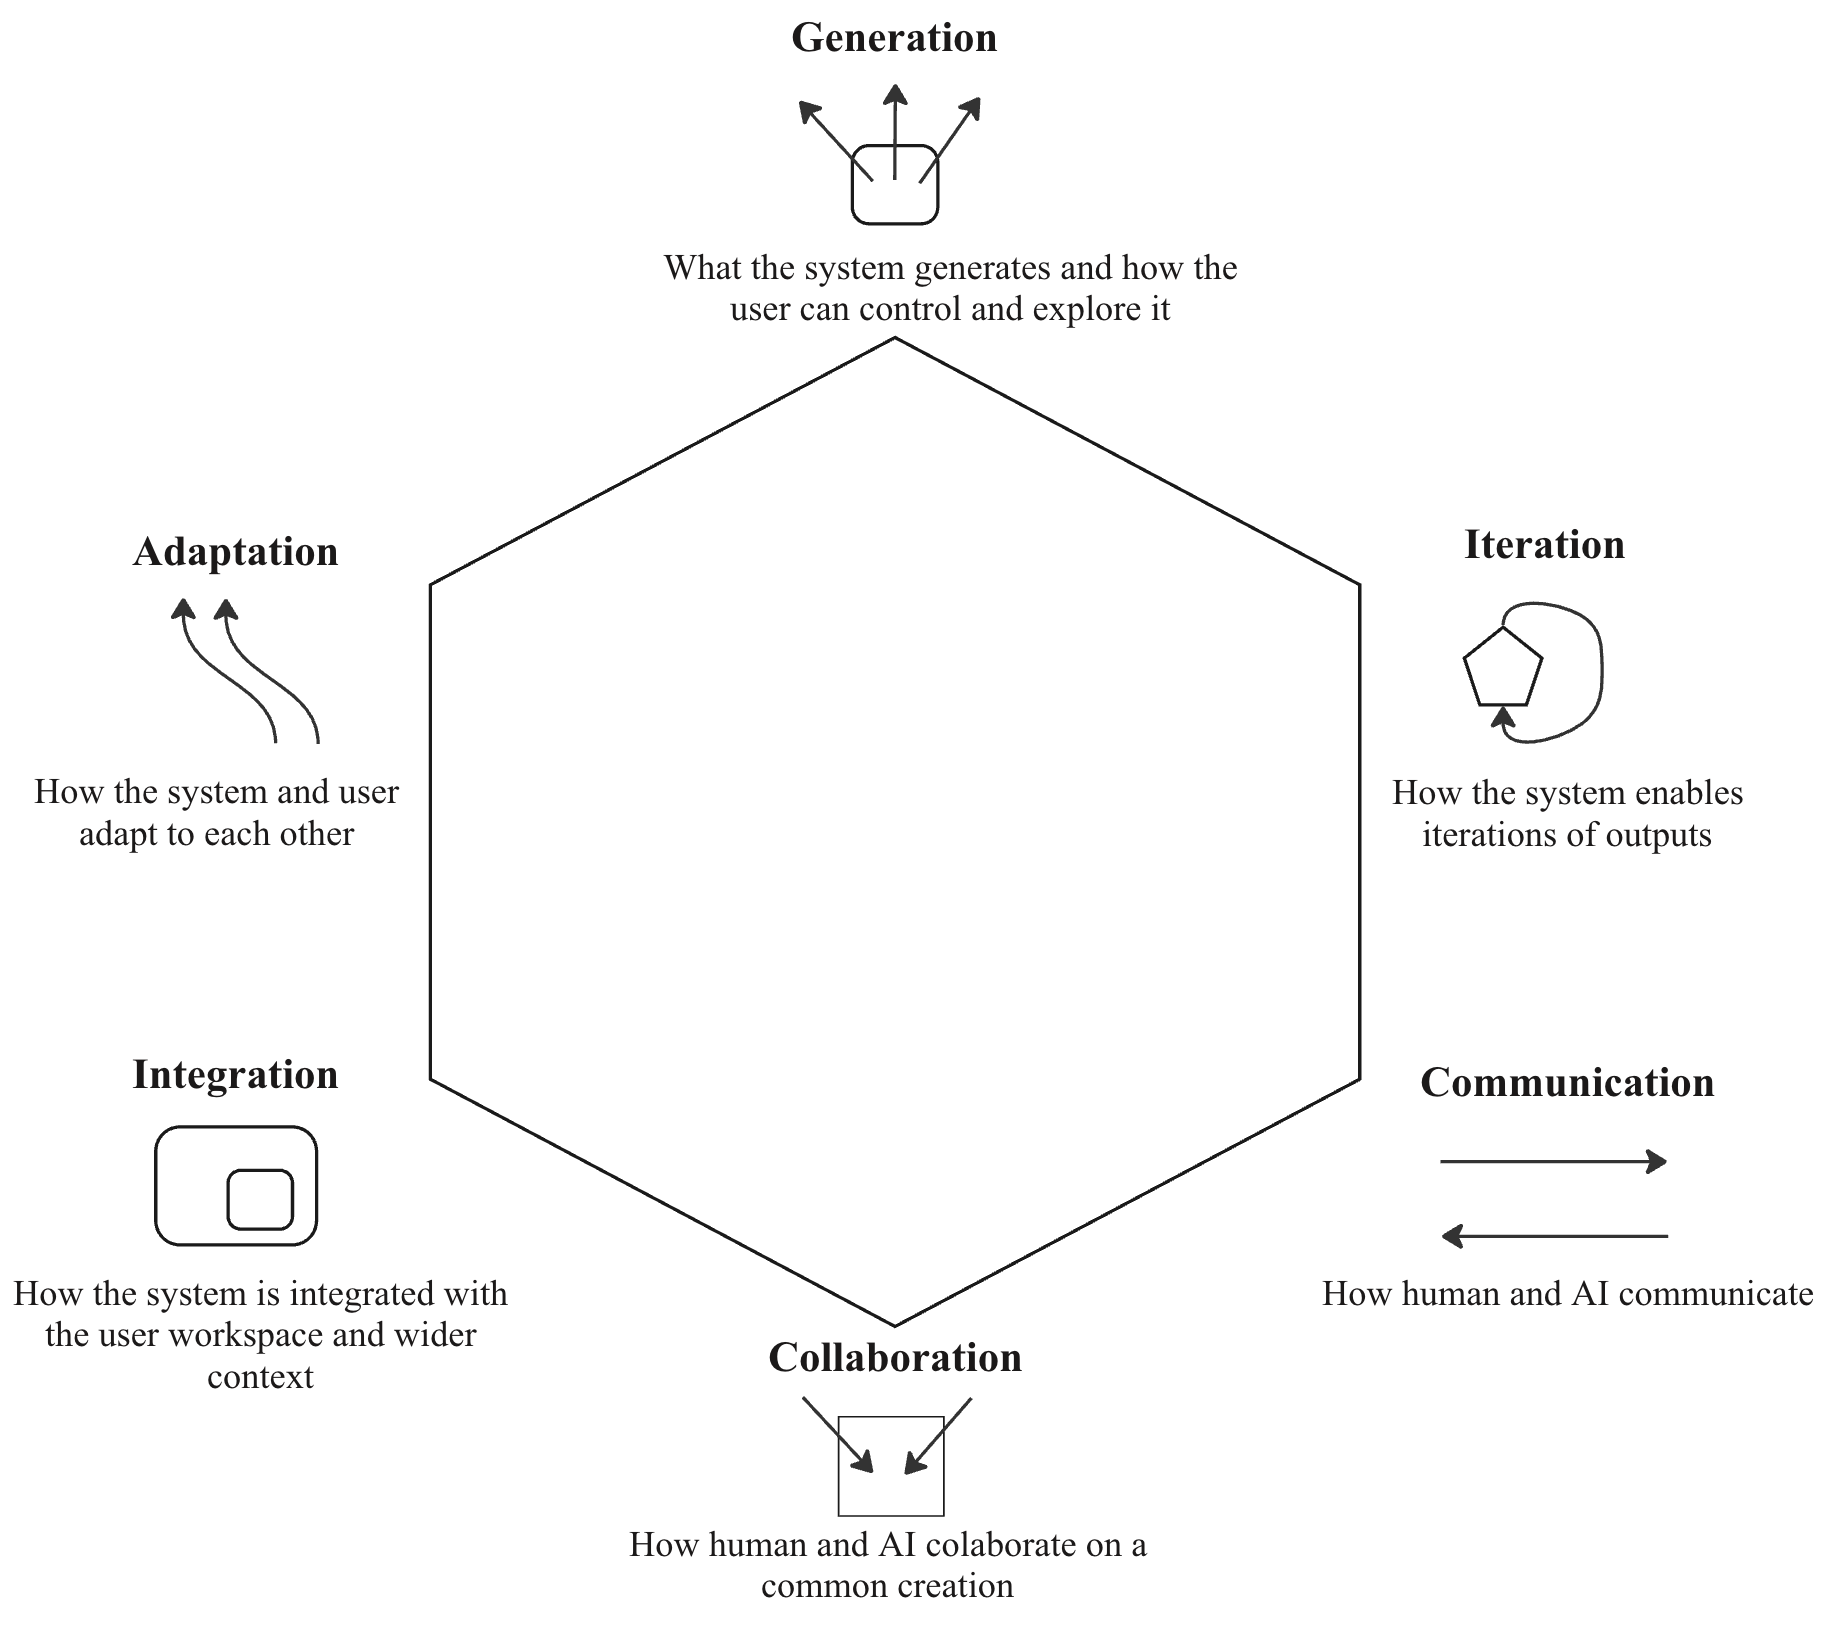
\includegraphics[width=1\linewidth]{sixdimensions.png}
    \caption{Six Dimensions of Human-AI Co-Creativity}
    \label{fig:sixdim}
\end{figure}

At a high-level, designing across each dimension fundamentally means asking the following questions for each:

\begin{itemize}
    \item \textbf{Generation: }Does the AI produce quality content, and can the user meaningfully control and explore the generative space?
    \item \textbf{Iteration: }Can the AI effectively support the iterative nature of the creative process?
    \item \textbf{Communication:} Can both the human and AI communicate effectively about goals and intentions to establish a mutual understanding?
    \item \textbf{Collaboration:} Can the human and AI able to collaborate effectively and contribute meaningully to the creative artefact?
    \item \textbf{Integration:} Does the AI integrate effectively into the user’s workspace, workflow and wider sociocultural context?
    \item \textbf{Adaptation:} Does the AI adapt to the user, and does the user adapt to the AI, evolving towards a deeply personal co-creative partnership?
\end{itemize}

In order to assess what \textit{meaningful} may mean, and how \textit{robustness} could be assessed, across each dimension, I introduce a set of design principles, each specific to a particular dimension. But first, I will discuss what each dimension entails and why each is distinctively relevant. 

\subsubsection{Generation}

The generative dimension is concerned with what the AI generates, the quality of its output, and how effectively the system enables users to control and explore this generative space. Considering the quality of generation as an important factor might initially seem trivial. However, when one considers that what is considered a quality output depends on the context and user preference, this acquires new significance. Moreover, \textbf{in co-creative systems}, the production of novel, interesting, or valuable content is not only in \textit{the eye of the beholder} but \textit{in the hands of the beholder}. An effective prompt or thoughtful combination of inputs by the user leads to compelling content, whilst a generic or poorly considered prompt may yield unremarkable results.

I observed this phenomenon in my Narrative Device experiment. Though the stories generated were not particularly riveting or can be considered of high literary merit, users nonetheless reported considerable enjoyment when using the system. This was partly due to the system surpassing their expectations—most participants had never previously interacted with a language model and were unaware of their capabilities. More significantly for this argument, the stories emerged from users inputting two different words or concepts that the AI then integrated into a narrative. This process involved users engaging in their own creative ideation to identify concept pairings that might yield interesting and enjoyable stories.

Moreover, a growing body of empirical research demonstrates that the perceived value of generative outputs in co-creative processes is inextricably linked to how users can both produce and explore the possibility space. Davis et al. found that designers engaged in ideation phases with image generation models expressed preference for GAN-based systems that facilitated navigation through a visual possibility space, as compared to diffusion text-to-image systems lacking this navigational metaphor—even when the latter produced technically "higher-quality" images \cite{Davis2024-ml}. 

Similarly, Park et al. documented that creative practitioners frequently find text-based inputs constraining, particularly in visual domains, as many self-identify as visual thinkers who struggle to articulate precise textual descriptions of their conceptual intentions \cite{Park2024-gw}. This cognitive disconnect between visual thinking and verbal description has prompted exploration of multimodal input systems that accommodate diverse cognitive and creative processes. The affordances of such systems appear to better align with the non-linear and often tacit nature of creative cognition.

This observation resonated strongly within my own writing experiments (Chapter 4), where participants consistently expressed desire for capabilities to incorporate images and other media formats to guide textual generation. Their reflections revealed a perceived limitation in text-only interactions, suggesting that multimodal inputs would have enabled them to produce more nuanced and satisfying content by leveraging complementary representational systems. This points to an important insight: generative capabilities must be conceptualised not merely as technical implementations but as \textit{generative interfaces} between human cognitive processes and computational systems.

\subsubsection{Iteration}

As generative capabilities have matured and AI systems have become integrated within diverse creative workflows, a fundamental limitation has persistently constrained their co-creative potential: the capacity to support genuinely iterative processes that accommodate both divergent exploration and convergent refinement. This limitation has crystallised into a distinct dimension of analysis—one that intersects with yet remains conceptually separate from purely generative considerations. The iterative dimension of co-creative AI systems invites critical examination of a foundational question: to what extent can these systems authentically support the inherently cyclic and non-linear nature of creative development?

This dimension's challenges manifested consistently across my empirical investigations. In the Australian Financial Review case study (Chapter 7), creative directors repeatedly encountered a constraint: they would generate compelling visual content but found themselves unable to selectively modify specific elements while preserving others. This iterative limitation stems from the fundamental architecture of generative models, which are optimised for producing complete outputs rather than targeted modifications. The resulting generation of entirely new content during attempted refinements created significant friction in the creative process, as I documented in my analysis of how iteration and consistent refinement—maintaining stability in some elements while enabling controlled modification of others—constitutes a critical limitation in the co-creative application of generative systems.

Recent technical developments have attempted to address this iterative constraint, particularly in visual domains, through methodologies such as in-painting, outpainting, guided edits, and feedback loops with ControlNet architectures. While these approaches have introduced limited iterative capabilities, they remain insufficient for supporting intuitive creative workflows. As of this writing (though technological developments may soon alter this landscape with the emergence of omnimodal models), no system reliably supports even basic iterative scenarios such as generating an image of an automobile and subsequently modifying specific attributes—converting it to an open-top model or changing its color—without substantially altering other visual elements that users wish to preserve.

The language domain exhibits comparatively advanced iterative capabilities, permitting multiple rounds of feedback and revision. However, significant challenges persist in facilitating nuanced, non-destructive editing or substantively redirecting a model's generative trajectory \cite{Bown2024-yx}. This limitation was articulated by participants in my writing study (Chapter 4), with one observing: "ChatGPT will always rewrite the entire passage to change just one paragraph, and it's harder to work on one text because I often need to scroll back up or continually copy and paste it." Another participant noted the difficulty in course-correction: "it's gone in the wrong direction and requires a lot of input from me to get it back on track."

These empirical observations reveal that iteration represents not merely a technical challenge but a conceptual reconfiguration of how we understand creative processes in human-AI collaboration. The capacity for meaningful iteration—with its embedded practices of reflection, refinement, and recalibration—functions as a critical determinant of co-creative potential. This dimension thus emerges as a crucial analytical lens through which we can evaluate the evolving landscape of generative AI systems and their capacity to support authentic creative partnerships.

\subsubsection{Communication}

The communication dimension emerged as a core element in my conceptualisation of human-AI co-creativity from the beginning of my research. Early on, I examined whether an early language model—not explicitly designed for dialogue—could be repurposed to support interactive communication that transcended mere content generation. Specifically, I was interested in exploring the model's capacity to engage not only \textit{through} creation but also \textit{about} the creation, and found evidence for both potential and limitatios to transition between these modes of engagement to discuss goals, preferences, feedback, and clarification at a meta-level while simultaneously co-authoring narrative content. This early exploration established communication as a critical analytical lens that addressing fundamentally, the following question: Can both the human and AI communicate effectively about goals and intentions to establish a mutual understanding?

Generally models, particularly in the language domain, have greatly improved in their communicative capabilities: it is now commonplace to engage with them somewhat fluid conversation across textual and auditory modalities. However, it would be reductive to consider meaningful co-creative communication as solved. 

For example as we showed in a paper I co-authored (though not as first author, thus not included as a primary contribution in this dissertation), even sophisticated AI language models encounter persistent difficulties in comprehending nuanced human intentions, particularly those involving humour and sarcasm. More fundamentally, contemporary models are not architected to engage in dialogue that progressively builds mutual understanding; rather, their communicative affordances frequently function primarily as mechanisms for fulfilling requests, since that is how they are evaluated \cite{Ouyang2022-af}.

Alternative communicative paradigms have begun to emerge in recent research. Moving beyond the prevailing assistant-request framework, some approaches have demonstrated promise by reconfiguring AI systems as thought provokers that pose questions to users—both to cultivate deeper understanding of user intentions and to facilitate users' own insight development \cite{Kim2023-wt}. More recent approaches seek to move away from subservient modes of communication that reinforce user views, and instead prioritise openness, curiosity, and willingness to offer oblique or even challenging viewpoints \cite{Anthropic2024-ne}.

Moreover, communication need not occur exclusively via language. Humans engage in rich communication beyond verbal exchange. Particularly in creative scenarios, they use subtle body language cues, signals, and sounds to communicate intentions and preferences. AI offers considerable unexplored potential here.

Rather than seeking anthropomorphic modes of communication, AI may offer new possibilities unavailable in human-human co-creativity. Engaging with new interfaces to communicate intent, from GUIs to brain-computer interfaces to embodied interaction, offers promise. Participants in my study documented in Chapter 4 consistently expressed desire for GUI elements that would enable communication with AI systems beyond written language. Other suggestions involved incorporating voice and multimodal inputs as channels for expressing intent and enable steering. 

While AI has undoubtedly progressed in approximating human-like communication, the achievement of substantive shared understanding—expressed both through and beyond language—remains an active research area and a conceptually rich dimension for consideration in human-AI co-creative system design.

While AI can increasingly communicate in human-like ways, achieving meaningful shared understanding remains an active area of research and practice. This includes enabling mutual understanding both through and about the creation, as well as exploring beyond-human modes of communication. As such, it provides a rich dimension to consider in the design of human-AI co-creative systems.

\subsubsection{Collaboration}

Chapter 4 began with the observation that prevalent chat interfaces, while facilitating communication, remain limited for collaborative work—primarily because they lack a shared space where both human and AI can contribute to an evolving artifact beyond the confines of the chat itself. This began delineating collaboration as a distinct dimension from communication. 

Indeed, my study revealed that chat interfaces tend to position users in less collaborative roles, primarily as instruction providers. Collaborative editors that enable interaction through creation can partially address this limitation and offer promising avenues for more balanced human-AI collaboration. Recent commercial developments, such as ChatGPT's Canvas, have begun implementing shared workspaces to foster more fluid collaborative processes.

However, the research also uncovered complexities in enabling meaningful collaboration even with these collaborative interfaces. Users expressed confusion about interface functionality and desired clear highlighting of AI contributions following edits. They emphasised the need for comprehensive version control and improved visibility of system affordances across both collaborative and communicative elements—highlighting that effective collaboration requires more than simply a shared space.

Notably, regardless of whether using chat-based or collaborative interfaces, users demonstrated a tendency to adopt directive approaches, having AI perform the "heavy lifting." This pattern aligns with observations throughout the literature regarding the roles humans typically assume when working with AI: less directly engaged and more instructional \cite{Palani2024-on}. Such interaction patterns are associated with skill atrophy and diminished creative self-efficacy, potentially undermining the beneficial aspects of co-creativity \cite{Lee2025-dw, McGuire2024-im}.

The rich literature on human-computer collaboration—spanning mixed-initiative systems, human-robot ensembles, and agent systems—documents complexities beyond those identified in this research. These include considerations ranging from automation bias to coordination challenges and explainability requirements \cite{Wang2020-cw, Horvitz1999-wh}. 

As such, collaboration thus represents a crucial and distinct dimension to consider when designing co-creative AI, essentially considering the question: Can the human and AI able to collaborate effectively and contribute meaningully to the creative artefact?

\subsubsection{Integration}

As AI is increasingly adopted as a co-creator, a critical consideration involves integrating these co-creative systems within users' workflows, workspaces, and contexts.

Consider the growing adoption of AI as a "pair programmers" and "teammates" in software development \cite{Cursor2024-ow, Ai2025-wi}. For these systems to effectively fulfil this role, they  require awareness of existing codebases and direct integration into developers' environments. Co-creative applications like Cursor, v0, and GitHub Copilot have gained traction largely because they embed AI co-creators within established workflows, and are well integrated within their main workspaces.

In visual domains, integration may mean that AI capabilities are embedded within graphic design and image editing software. Platforms like Canva and Adobe Photoshop are beginning to integrate AI capabilities within the software and within established workflows, which is not a trivial task. This does not only involve embedding it into the software, it also involves being aware of previous previous work, including brand kits, portfolios and guidelines, such that it can generate content align with this. The need for visually aligned work was observed in both of my case studies presented in Chapter 6.

Integration may also mean integrating with other generative toolsas increasingly, a burden for the potential of co-creative AI is a fragmented ecosystem \cite{Palani2024-on}. This was particularly evident in my AFR case study (Chapter 7), where our image creation process necessitated movement across multiple disconnected systems. We generated initial style and content references in one generative application, created target images with these references in another, performed in-painting modifications in a third, and completed final retouching in a conventional non-generative editor. Similarly, a limitation of Tilly as a design co-creator was that it was not connected to material sourcing software, an important and often considered tedious part of the job. 

Integration also requires situated awareness within broader sociocultural and environmental contexts. A co-designer might consider seasonal trends and material sustainability. A co-creative writer may need to consider the larger sociocultural and political context, as some participants expressed in my writing study. Such contextual integration was central to my two installations from chapter 5. Music of the Sails involved integrating the AI co-creator with building data and a music generation engine. System of a Sound integrated local, national economic, and global atmospheric data to produce contextually responsive generative art. 

As AI co-creators become more pervasive, considering how they integrate within immediate workspaces, and wider sociocultural contexts becomes a crucial dimension for consideration. 


\subsubsection{Adaptation}

A final consideration is how AI co-creators adapt to users. Each user has a distinct creative process, preferences, collaboration style, expertise, and personality. Consequently, an important question arises: does the AI adapt to the user, and does the user also adapt to the AI, evolving into a deeply personal co-creative partnership? Compared to the other dimensions, this area remains relatively unexplored and may pose greater technical challenges.

Moruzzi \cite{Moruzzi2024-cq} recently introduced an approach to enable user adaptation and personalisation in co-creative agents. In this framework, users can adjust parameters such as level of expertise and communication style to tailor the system to their needs. In my own research, a recurring theme was the desire to personalise outputs so they align with a user’s style. For instance, in the Tilly project, the aim was not only to match the studio’s aesthetic but also to co-evolve a distinctive aesthetic that could serve as a long-term asset. To support this, we implemented a Retrieval Augmented Generation mechanism that allowed Tilly to learn from interactions over time, accumulating knowledge from both in-studio designers and external experts.

Commercial systems are now beginning to offer forms of personalisation and adaptation. ChatGPT, for example, uses a memory component that learns user facts and preferences, while Midjourney’s moodboards allow users to cultivate unique styles, and Leonardo supports LoRa training for personal model fine-tuning. However, co-creative adaptation is still in its infancy. One can imagine a future where individuals collaborate with uniquely tailored co-creators that are highly attuned to their creative processes, strengths, and areas for growth.

Notably, adaptation should occur in both directions: the system learns from the user, and the user (or team) adapts to the system. Over time, this mutual adjustment could enable what Blanchard \cite{Blanchard2024-jz} terms “symbiotic virtuosity”: a personal, evolving relationship with a co-creative AI that pushes creative skills and intentions to new directions.

\section{A framework for Human-AI Roles in Co-Creative Systems}

Having established the six dimensions of co-creativity that I explored throughout my thesis, and that I propose are crucial to consider in designing co-creative systems, I want to now turn my attention to another critical component of co-creative systems: the role that humans and AI play in co-creativity.

The significance of role allocation stems from the observation throughout this thesis that AI does not assume a monolithic co-creator role, but rather manifests in various nuanced capacities that emerge in different contexts. This observation aligns with existing literature, which will be discussed further in this section.

As discussed in the preceding chapters, the roles adopted by humans and AI in co-creative systems depend on several factors:

\begin{itemize}
    \item User preferences and their willingness to engage in or automate specific tasks
    \item Interface/interaction design and technology affordances that predispose both users and AI toward particular roles
\end{itemize}

For example, in the narrative device case study discussed in Chapter 4, which produced short stories by combining two user-provided terms, participants predominantly utilised the system for ideation, generating prompts for their own subsequent writing. In contrast, when using prototypes that enabled a collaborative editor with integrated chat functionality—while employing fundamentally the same underlying model—participants more frequently engaged the AI system during convergent stages, primarily for polishing and editing their texts. Furthermore, participants using a version of the same prototype with a chat-only interface assumed more directive roles, providing instructions for the AI to execute the writing while remaining less involved in producing actual text themselves.

These examples illustrate how the same fundamental technology—a Large Language Model (LLM)—led to systems assuming different co-creative roles based primarily on interaction design. While individual variability influenced how participants utilised AI and the tasks they assigned to it, trends in role assumption emerged as a function of the interaction paradigms afforded by each system.

How can we systematically understand the different types of roles that emerge and how interaction paradigms affect them? This question drives the analysis presented in this section, which constitutes one of the three core contributions of this thesis.

\subsection{Spaces and Stages Model: A Framework for Co-Creative AI Roles}

This section presents the Spaces and Stages model—a simple yet powerful framework for characterising the types of roles co-creative AI may assume within a creative process. Numerous role characterisations have been proposed in the literature \cite{lubart, kantosalo}. Lubart categorizes AI as penpal, coach, or nanny; Maher describes roles that support, enhance, or generate; and Nakakoji classifies systems based on whether they help users accomplish tasks faster, train skills, or enable entirely new forms of creativity akin to novel instruments.

However, these existing frameworks offer limited discussion of how these roles are determined or adopted in practice. Moreover, they focus primarily on assigning categorical labels to different roles. Rather than proposing another set of specific role labels, which is indeed useful, this framework provides a meta-level conceptual structure within which different roles may be situated and understood in relation to the creative process.

\subsubsection{Spaces}

A crucial distinction explored throughout this thesis is the concept of interaction occurring both \textit{through} and \textit{about} the creation. Interaction \textit{about} the creation encompasses discussing goals, preferences, intentions, clarifications, and feedback, while interaction \textit{through} the creation involves acting directly upon the shared artifact—providing words in writing, drawing lines in visual arts, etc.

This distinction has been a recurrent theme throughout this research, introduced in detail in Chapter 3, where early versions of language models were explored for their capacity to enable such interactions. That chapter proposed a set of possible actions that can be taken in co-creative dialogue by both human and AI, primarily divided between those occurring through and about the creation. Similar distinctions have been proposed by \cite{rezwana} and \cite{kellas}.

This conceptual separation was further empirically investigated in Chapter 4's second paper, "Beyond chat: towards greater user involvement and agency through shared collaborative spaces," which focused on understanding the effects of interfaces that facilitate interaction both through and about the creation, versus those that primarily enable interaction about the creation, such as chat interfaces.

Building upon this distinction, creative processes can be understood as involving actions within two spaces:
\begin{itemize}
\item \textbf{Abstract space}: Where users develop ideas, goals, and intentions at a higher level of abstraction
\item \textbf{Execution space}: Where users act directly on the creation—writing actual words, drawing lines, or playing musical notes
\end{itemize}
\begin{figure}
\centering
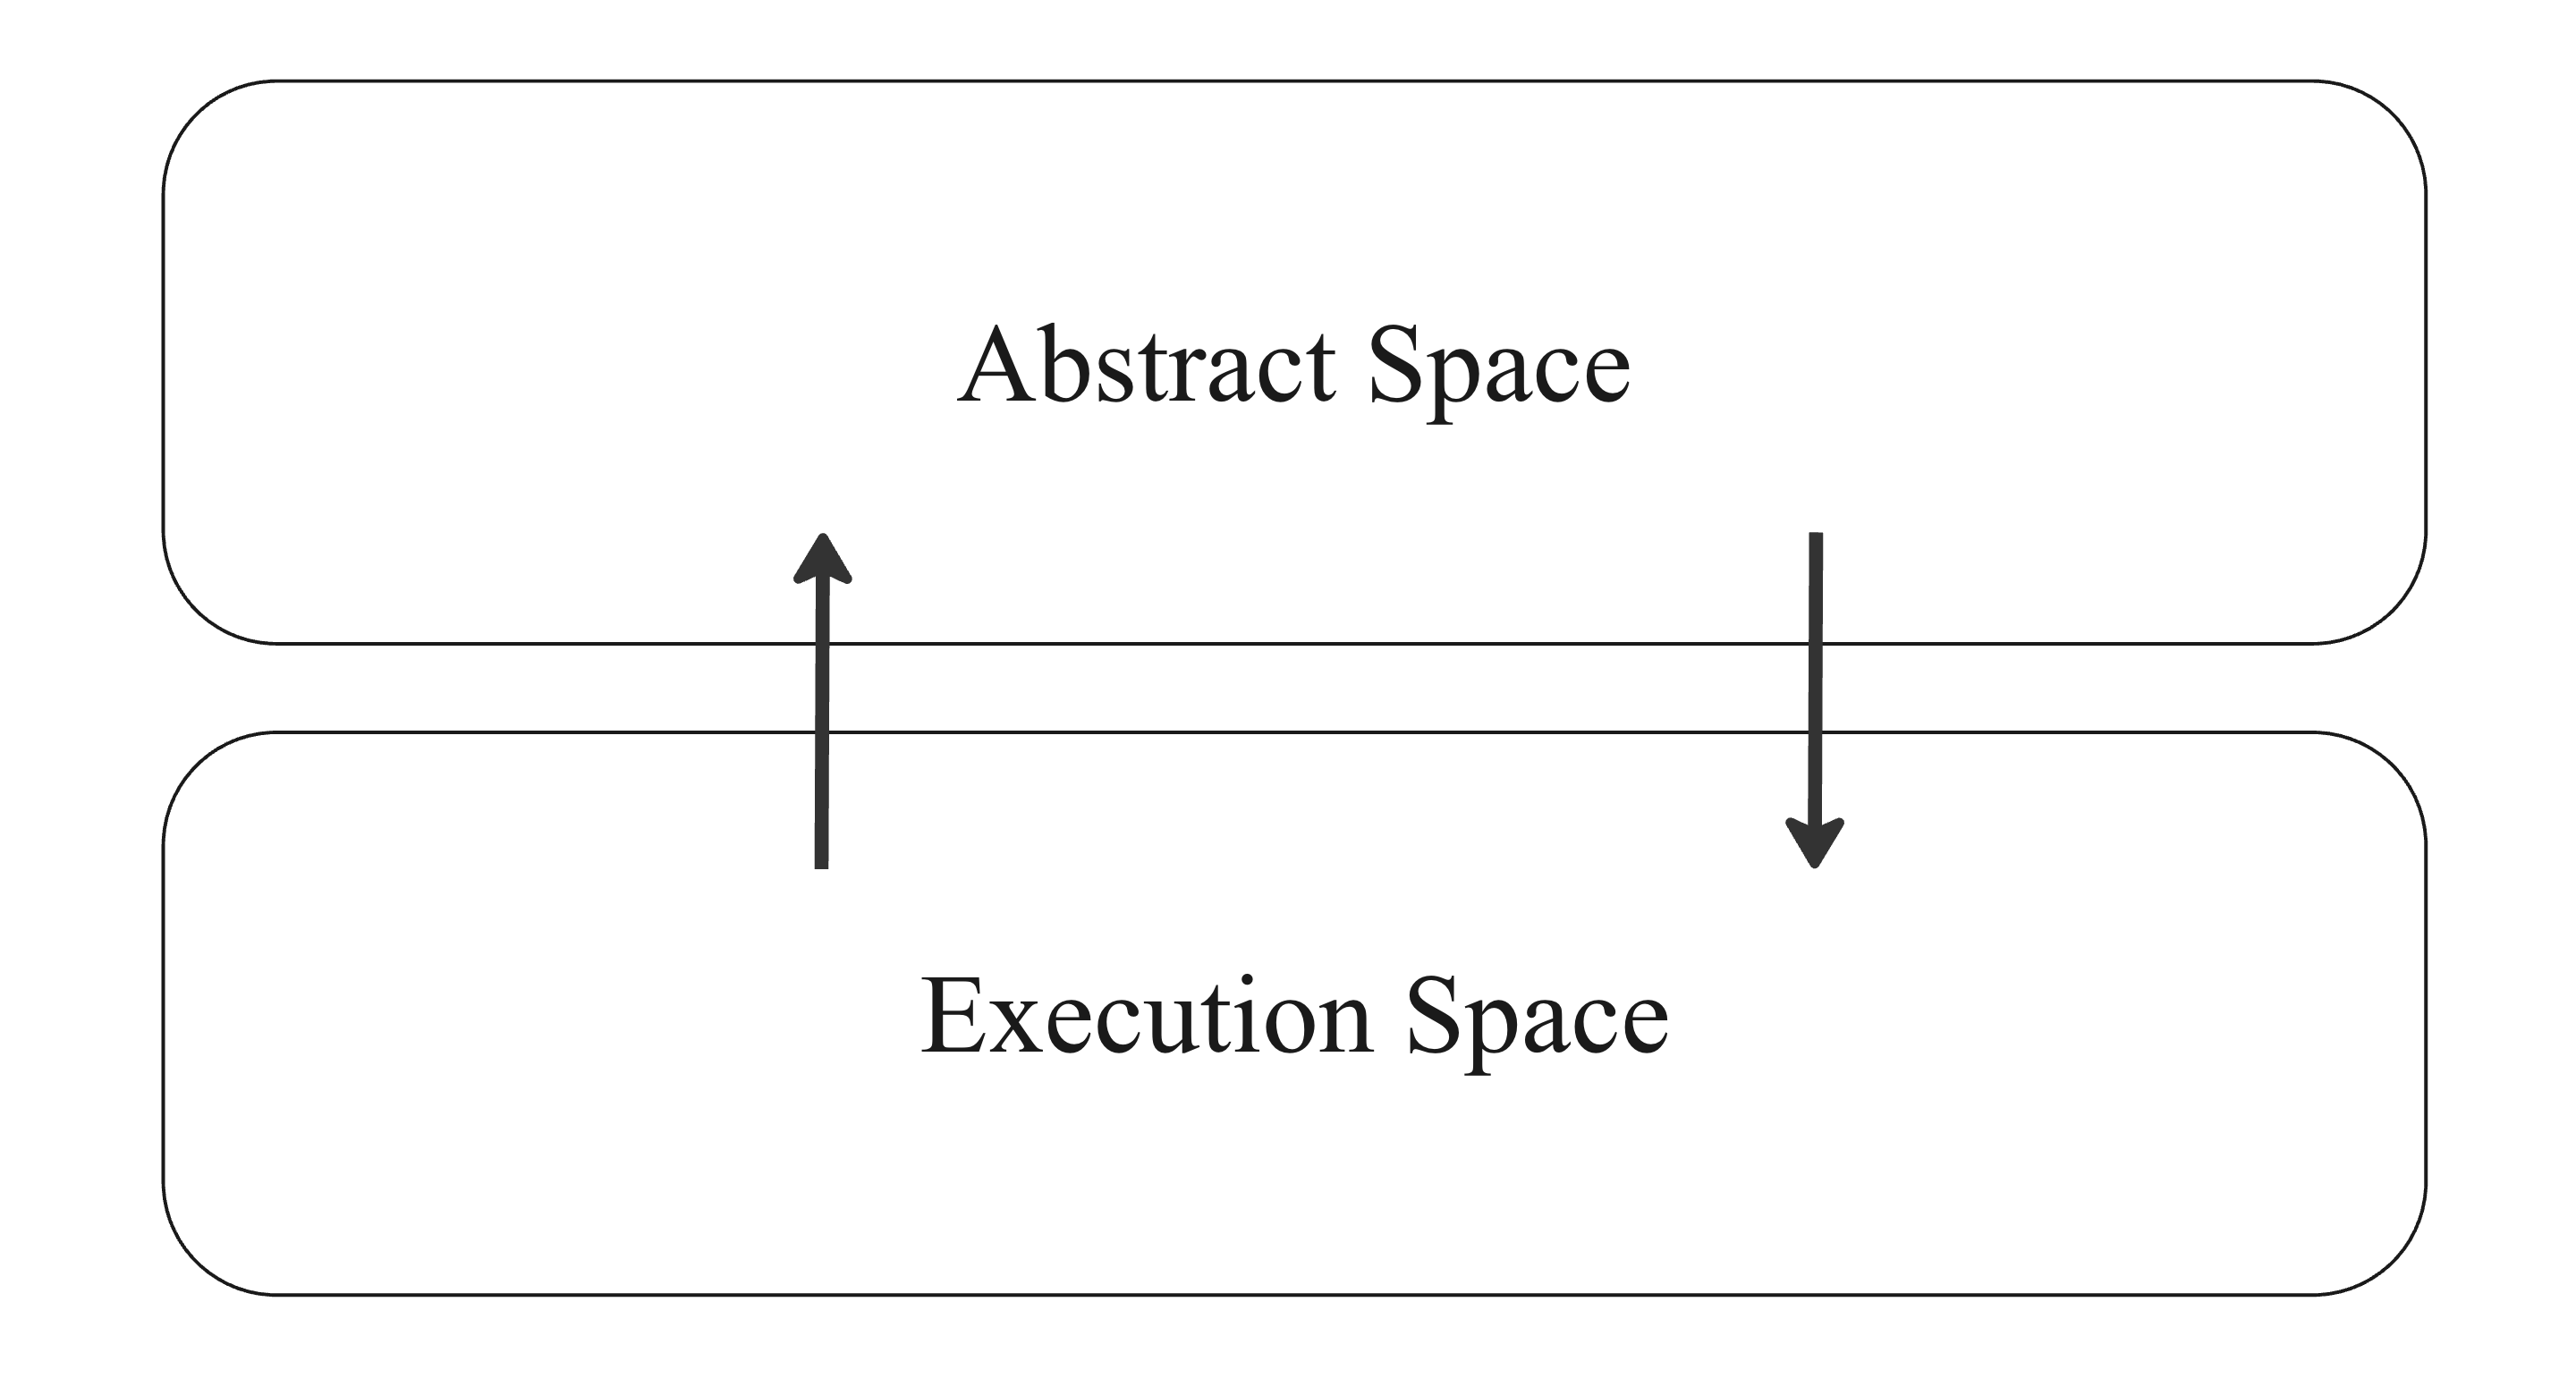
\includegraphics[width=1\linewidth]{twospaces.png}
\caption{Creative Processes Involve Moving Between Abstract Spaces and Execution Spaces}
\label{fig:enter-label}
\end{figure}

Creativity is largely a process of formulating ideas and intentions in the abstract space, then transitioning to the execution space to realise them. This process rarely follows a linear trajectory; instead, it typically involves iterative movement between these spaces. Actions in the execution space generate new concepts in the abstract space—including value judgments and novel ideas—which are subsequently explored further in the execution space, establishing a continuous, and often very tight, feedback loop between abstraction and execution.

This distinction offers a simple yet effective way to conceptualise human-AI co-creative roles. An observation from both this thesis and the broader literature is that, at least under current interaction paradigms, users tend to migrate toward higher levels of abstraction, like ideating and planning, while outsourcing tasks at the execution level to the AI, such writing words, code or drawing pixels. Indeed, it often said both by commentators and even AI companies that the value of AI "reducing the gap between idea and execution".

This arrangement presents certain advantages, enabling individuals to realise their creative ideas even when they lack specific technical skills or resources. For instance, a person may conceive compelling ideas for films or short stories but struggle with the writing process itself. However, this division of labour, where users adopt primarily directive and ideation roles in the abstract space, may potentially erode skills and self-efficacy, ultimately diminishing creative satisfaction.

An illustrative example was provided by a participant in one of the studies discussed in Chapter 4. When describing how Vorges, the co-creative AI, performed most of the writing while they provided the ideas, they stated: "[it] made me feel like I was cheating somehow. It does not feel like my work, even though I gave all the ideas. Also, I believe there is satisfaction in putting a lot of effort/dedication/patience into something. Vorges made everything so simple, fast, and easy that it felt artificial and no real satisfaction came as a result." Another participant claimed their role was "like giving the recipe of a cake to someone and letting it do it."


In an extensive survey of roles assumed by humans and generative AI, \cite{Palani2024-on} describe users describe themselves as "ideators and project managers with a larger creative vision orchestrating information context and tasks across multiple GenAI models instead of traditional workers executing each task". 

However, this means that users are generally becoming less involved at execution levels. An emerging trend in coding, for example, which Andrej Karpathy has termed "vibe coding", involves: 

\begin{quote}
"[I] forget that the code even exists. It's possible because the LLMs (e.g. Cursor Composer w Sonnet) are getting too good. Also I just talk to Composer with SuperWhisper so I barely even touch the keyboard. I ask for the dumbest things like "decrease the padding on the sidebar by half" because I'm too lazy to find it. I "Accept All" always, I don't read the diffs anymore. When I get error messages I just copy paste them in with no comment, usually that fixes it. The code grows beyond my usual comprehension, I'd have to really read through it for a while. Sometimes the LLMs can't fix a bug so I just work around it or ask for random changes until it goes away. It's not too bad for throwaway weekend projects, but still quite amusing. I'm building a project or webapp, but it's not really coding - I just see stuff, say stuff, run stuff, and copy paste stuff, and it mostly works."
\end{quote}

While this can be considered a natural progression of coding, moving to higher levels of abstraction, research suggest this reduced involvement and diminished cognitive effort can lead to more errors and loss of cognitive skills \cite{Lee2025-dwL} Instead, some practitioners propose a more productive and long term beneficial approach involved engaging iteratively with the model \cite{Osmani2024-br}. 

Indeed, while AI itself, as a cognitive automation technology may offer a path of least resistance towards less involvement at the execution space, interaction design can also significantly impact this. For example, the participants in my study who reported less involvement were using a control version of the co-creative system which only enabled interaction via chat, primarily leading the user to adopt tasks in the abstraction space: giving ideas, feedback, and value judgements. In contrast, a user employing a version of the tool enabling both collaborative editing and chat, who reported engaging deeply in writing at the execution space, observed: "It forced me to put in some effort and do the majority of the work, I enjoyed how I could not be fully reliant on AI to provide me with all the text." Another participant using the same version claimed: "I really-really enjoyed writing this. I even had a deep moment of reflection, my writing was nostalgic and sad, but I was able to use AI to steer it in the right direction, it gave me confidence that I was also writing with correct grammar and spelling, English is not my first language and while I am proficient, I can still use proofreading to ensure good quality." Both of these participants, reported they did most of the work but AI helped them with suggestions, editing and other supportive tasks. 

These contrasting experiences highlight what I propose may be \textbf{fundamental tension of human-AI co-creativity}:

\begin{quote}
    As AI can increasingly assume complex roles within the creative process; users tend to move up levels of abstraction and adopt more directive roles, while they outsource execution-level roles to the AI. On one hand, this can help augment human creativity by helping them realise their ideas faster and with less resources. On the other hand, it may hinder their creativity by increasing errors, reducing quality, and eroding critical creative skills, agency, and satisfaction.
\end{quote}

When designing co-creative systems, designers, developers, and researchers must consider this \textbf{fundamental tension in human-AI co-creativity}. A critical observation in my research and in the literature is that facilitating user engagement at both the abstract spaces and execution spaces may be an effective strategy to address this fundamental tension, helping them realise the beneficial co-creative potential of AI while reducing the shortcomings of increased creative and cognitive offloading. A promising alternative is enabling both collaborative spaces and communication spaces, where interaction through and about the creation are separated. However, how to effectively implement this in practice remains an important area for further research. 

\subsubsection{Stages}

A second conceptual dimension of the framework recognises that creative processes progress through different stages, with AI potentially assuming distinct tasks at each stage. Various stage-based models of creativity have been proposed in the literature, but for simplicity, this framework distinguishes between divergent and convergent stages.

A few examples from throughout this thesis offer an illustration of what factors may lead to the human and the AI to assume certain roles within each stage. For example, the designers working with Tilly in the case study described in Chapter 6 system initially utilised it to ideate novel designs for complex briefs both conceptually and visually—a divergent process—and found this application highly valuable. However, they encountered greater challenges during convergent processes, when they wanted to produce final renders, and editable files. Largely this was the result of limitations in the interface and the underlying generative model that failed at effective non-destructive iteration of outputs. It was also not fundamentaly able to produce 3D vector models which are considered the final stage of their process (before manufactoring). 

In creative writing participants in the "Beyond chat" study described in Chapter 4, employed AI primarily to polish drafts \textit{they had initiated}, thus engaging AI during a \textit{convergent} stage, mainly when they interacted with it throug both a chat and a collaborative text editor. In contrast, users of chat-only interfaces reported using AI as a brainstorming partner—a divergent application. 

Lastly, in the installation case studies described earlier, AI was utilised predominantly in convergent stages to execute performances, while the ideation stage remained primarily human-driven. This case, being a new type of creative practice, warrants further discussion that will be treated in later section.

\subsubsection{Spaces and Stages Integration}

Integrating these two dimensions produces a model with abstract and execution spaces on the vertical axis and divergent and convergent stages on the horizontal axis. AI roles can be roughly positioned within this grid, with the understanding that roles may shift over time, and AI can move between positions throughout a single interaction. In some cases, this movement occurs fluidly, while in others, the affordances of the tool may constrain the AI to a more fixed position.

\begin{figure}
    \centering
    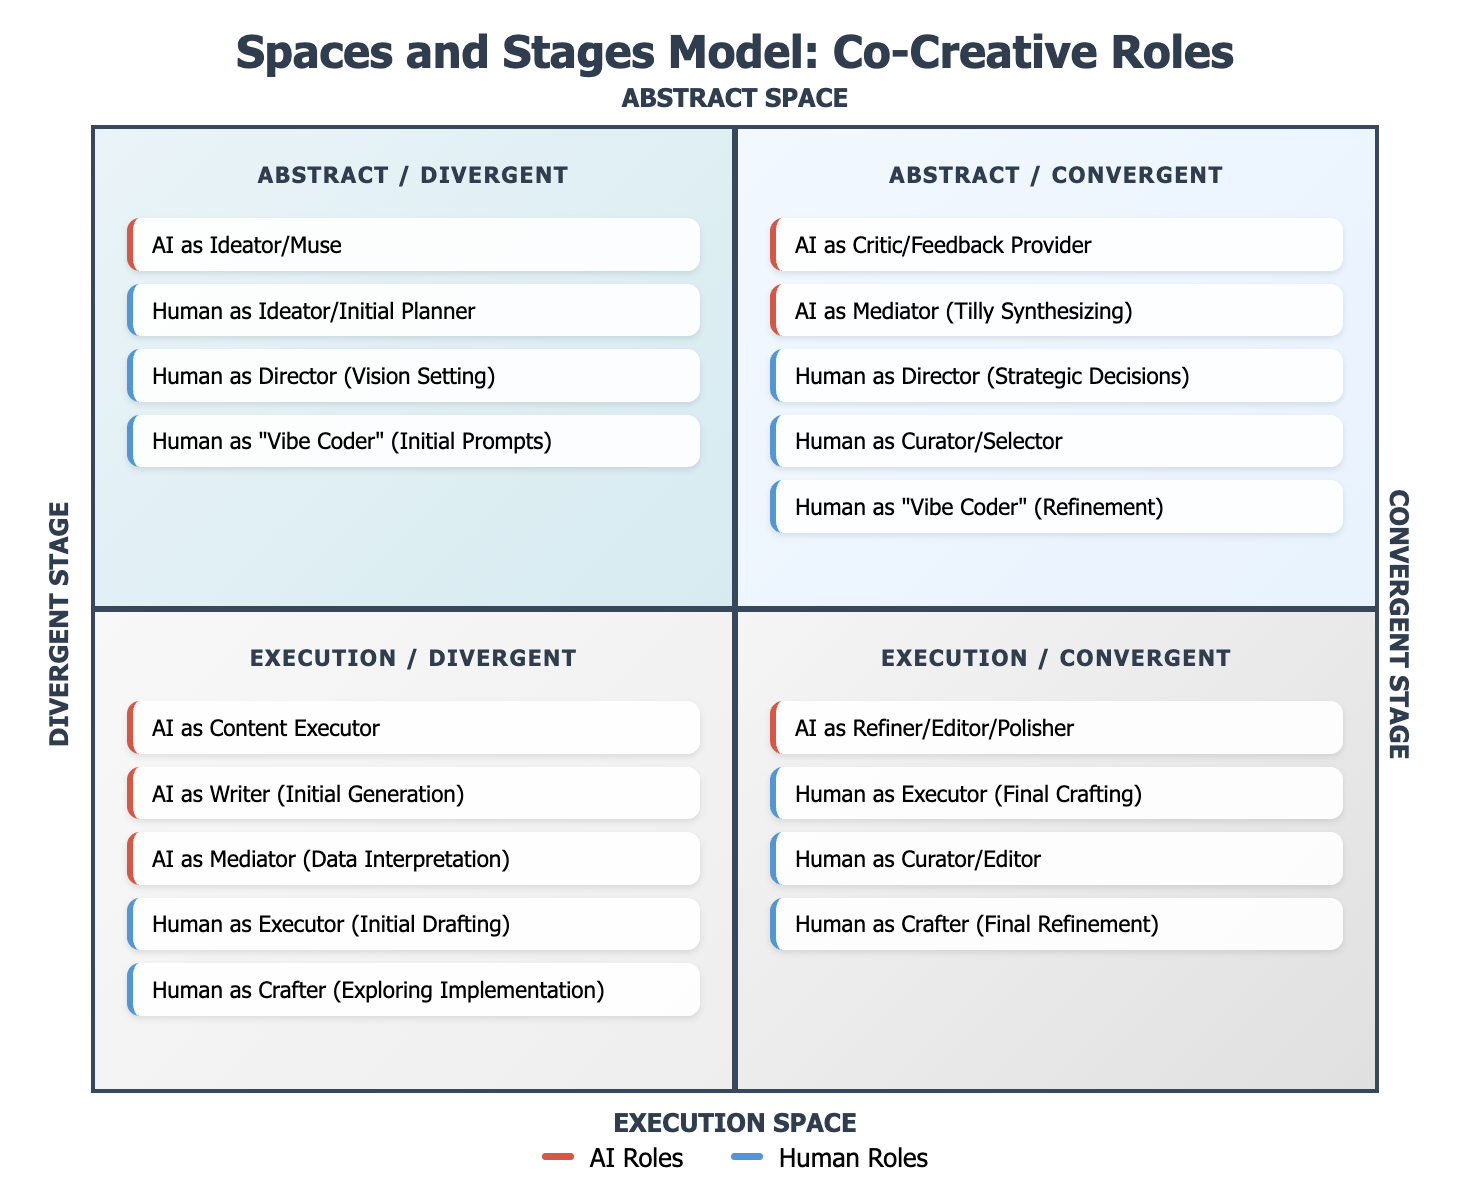
\includegraphics[width=1\linewidth]{spacesandstages.png}
    \caption{The Spaces and Stages model for co-creative AI roles. When developing a co-creative AI system one question designers and developers may ask is: where does my system sit within this model, and how does it allow users to move through it?}
    \label{fig:spacesandstages}
\end{figure}

The notion of spaces is well-established in creativity research and computational creativity literature, particularly in Boden's conceptual spaces theory, which was later formalised by Wiggins. While this thesis does not offer an exhaustive formalisation of abstract and execution spaces and their framing within Wiggings's conceptual space—leaving that for future work—it is worth noting that both can be understood within the broader framework of conceptual spaces.

In Wiggins' formalisation, conceptual spaces encompass both unrealised and realised artifacts, with a set of rules governing exploration and transformation between these states. Drawing a preliminary parallel, the abstract spaces proposed in this model can be understood as including both unrealised and realised artifacts at a conceptual level, while execution spaces may comprise the rules and mechanisms of exploration that facilitate the transition from unrealised to realised artifacts.

This distinction is important to the core argument made here: that both working at the abstract and execution level is important. It is useful for a creative to know the rules (execution space) for how to traverse the conceptual space they are working in and not merely act in the abstract space. For example, it is useful for a musician to know music theory, how to use scales, and how to play an instrument. While an AI may abstract this away, enabling a user to merely say: play an upbeat song, this will likely constrain their potential to meaningfully explore, and transform the space. This does not mean that knowing these rules is a prerequisite. In fact, not knowing the rules may be conducive to breaking them. However, within the observations in my research and in the emergent literature, AI automating the application of this rules, and the actions at the execution space presents a risk to effective co-creativity. 


\subsubsection{Narrow vs. General AI Co-Creators}

This framework is useful for another categorisation of roles which I offer here. Within each quadrant of the spaces-stages framework, different tasks can be located. A role corresponds to assuming one or more tasks within a particular region. Many previous role classifications were developed in a technological landscape where computational algorithms were constrained to specific, narrow tasks. However, newer generations of algorithms give rise to co-creators capable of moving across tasks and stages of the creative process, rather than merely automating isolated components.

For example, whereas earlier systems might focus exclusively on generating ideas, or merely generating an image, new emerging more capable systems can assist users across both abstract and execution spaces and across divergent and convergent stages level. I propose we are witnessing a gradual transition from narrow to general AI co-creators.

With this: I propose the following: 

\begin{quote}
    \textbf{A narrow AI co-creator} is a type of role that primarily occupies a fixed position within the Spaces and Stages Model, assuming specific and narrowly defined tasks, and which generally is not robust across the six dimensions of co-creativity
\end{quote}

\begin{quote}
    \textbf{A general AI co-creator} is a type of role that is high across the six dimensions of co-creativity, and which can engage with the user at the abstract and execution spaces, and across divergent and convergent stages. 
\end{quote}




\section{Design Principles for Human-AI Co-Creative Systems}

While multiple design principles have emerged across various domains, there are no specific design principles for co-creative AI systems. The most recent comprehensive effort by \cite{Weisz2024-io} establishes design principles for generative AI broadly, encompassing many applications. Within their six general principles, "Design for Co-Creativity" represents only one component.

As computing capabilities evolve, new usability principles become necessary. For example, the transition from terminals to graphical user interfaces required the development of new guidelines for interaction with computers, exemplified by Apple's Human Interface Guidelines first published in 1987, which have been regularly updated while maintaining core elements.

Now, as we transition to new modes of interaction with computers as a result of generative AI, particularly in the field of co-creativity, new principles that guide their effective development are needed. This need builds upon foundational work in human-computer interaction, including \cite{Horvitz1999-wh} principles for mixed-initiative interfaces, \cite{Resnick2005-fs} design principles for tools supporting creative thinking, \cite{Nielsen1994-df} usability heuristics, \cite{Norman2013-hs, Norman1994-kz} principles for everyday design and cognitive enhancement, and \cite{Amershi2019-vy} guidelines for human-AI interaction.

Each design principle proposed in this thesis corresponds to one of the dimensions identified in our framework and aims to provide robustness in that particular domain. Moreover, these principles can serve as metrics to evaluate how robust a system is across each dimension.

It is important to note that these principles will not apply universally to every system or use case. Their prioritization depends on the role the system assumes and the specific application context. The principles aim to be sufficiently general and comprehensive to allow developers of generative AI systems to select and adapt them to their particular scenarios, thereby providing a set of best practices for generative AI co-creative systems.



\subsection{Generative Dimension}

\begin{enumerate}

\item \textbf{Enable Meaningful Multimodal Control}

The idea that successful  interfaces  should  “provide  a  strong  sense  of  understanding  and  control" \cite{Donald1986-hx} has long been an important tenet in human-computer interaction design. This is particularly relevant for generative systems, which are often difficult to control. 

There has been considerable progress in enabling user control of generative AI outputs. For example, early systems that generally produced random outputs by sampling from a distribution \cite{Goodfellow2016-su} to modern approaches that produce outputs that adhere closely to natural language prompts, the current wave of AI adoption is largely a result of these capabilities. However, practitoners of these systems often express frustration with the "slot-machine" quality of outputs \cite{Nebelong2023-rb}, and the limitations of text-only interfaces. 

Multiple studies have shown that lack of perceived control is a common frustration expressed by users of generative AI systems. 
In my own research, the case study discussed in Chapter 6 \cite{Ocampo2024-dv} found that in the context of making production-level materials for a magazine, users wanted more control over the output than was afforded by the systems, such as controlling detailed aspects of the scene's composition style and other factors. 

Recently, a study by \cite{Park2024-gw} revealed that one of the main challenges expressed by professional creatives was working only with \textit{text interfaces} were perceived as too limited. Designers, who consider themselves visual thinkers, expressed a clear preference for interfaces that allowed visual inputs. Similarly, \cite{Peng2024-tr} found that enabling designers to use mood boards and images as guides led to a more nuanced expression of their creative intentions, thereby enhancing their sense of control. 

The ability to control output generation is central to effective co-creativity, as it empowers users to navigate the creative process while maintaining agency. Although current interfaces and models have made progress in aligning with user instructions and prompt adherence, they often fall short in facilitating control across multiple modalities. For instance, in a music generation system, allowing users to input musical examples rather than relying solely on text-based prompts could lead to more precise and contextually rich outputs.

This could also help people with disabilities, such as language and speech impairments, or different forms of thinking. 


\item \textbf{Allow for Serendipity}

Although user control is critical, \textit{serendipity} plays an equally important role in the creative process and can be one of the core strengths of generative AI in co-creativity. In a study on human-AI collaboration in drawing, users explicitly highlighted moments of serendipity as one of the most enjoyable and engaging aspects of the interaction. Serendipity is different from seeking novelty since a system might be explicitly tuned to do novelty search and diverge from known distributions, while serendipity might mean the happening of accidents instead. While designing for these accidents may be by definition hard (if explicitly designed, they may not be accidents), systems can be conducive to happy accidents occurring within it. For example, \cite{Koch2020-gx} reported that a cascading interface elements where users could browse images as conducive to serendipity, separately to the interface where they honed in chosen designs, stimulating ideation and finding things that were not being explicitly searched for. However, it is important to note that serendipity may not be adequate in convergent phases, where users may want to "get the job done". For example, in a study of human-AI co-ideation in design \cite{Chiou2023-vr} described how a user appreciated momnts of serendipity in an ideation phase, but found them frustrating in a convergent phase. 

    
\item \textbf{Enable Combinatorial Creativity}

The recombination of elements in novel ways is a fundamental aspect of creativity \cite{Boden1998-yn}. In my Narrative Device exploration, the system was designed to allow users to narratively combine two distinct concepts, which resulted in an organically used system that generated over two million stories. In other creative contexts, users frequently seek to merge disparate elements---whether combining aspects of an image, fusing styles in music, or integrating divergent ideas. A notable example is Google’s recent launch of Whisk, an image generation system that eliminates text inputs entirely, enabling users to generate images solely by combining two existing images. Such systems underscore the importance of designing for combinatorial creativity, where the integration of various elements is a deliberate and empowering feature.

    
\end{enumerate}


\subsection{Iteration Dimension: Design Principles}

\begin{enumerate}

\item \textbf{Facilitate Guided Exploration}

Creativity is largely a process a search and exploration \cite{Ritchie2012-nb, Wiggins2006-zd, Boden1998-yn}.  Renick et al's \cite{Resnick2005-fs} design principles for tools to support creative thinking, established the first principle as supporting exploration, arguing that "almost by definition, creative work means that the final design is not necessarily known at the outset, so users must be encouraged to explore the space". In modern generative systems, this process often involves exploring a latent space, and many approaches are being explored to enable this effectively \cite{Loh2024-fb, Smith2022-dm, Schaerf2024-gf}. This is a notably difficult problem that spans model interpretability and interface design. At the interaction layer, many current interfaces like text-to-X systems are biased to one-shot productions rather than navigation. Recently, Leonardo AI introduced Flow State, an interface that allow users to navigate a space of images without manually modifying the prompt. A recent study \cite{Davis2024-ml} found that such navigational image space, like those enabled by GANs \cite{Goodfellow2014-jz} better supported ideation than text-to-image interfaces in modern diffusion models. Adopting a navigational metaphor is a promising avenue for interfaces can better support users in exploring a broad spectrum of creative possibilities. Beyond graphical navigation, \cite{Resnick2005-fs} argues that an important component of enabling search and exploration is allowing users to try different things and backtrack when needed, as well as maintaining rich histories of past interactions.   

\item \textbf{Create Feedback Loops}

Facilitating a process in which outputs are reintroduced as inputs enables self-reinforcing feedback loops that can drive the creative process forward. Moreover, this can be one of the distinctive strengths of generative AI systems. For example, writer Robin Sloan \cite{Sloan2016-fj} developed a custom system using a recurrent neural network embedded within his writing editor. This system allowed AI-generated autocomplete suggestions (or his own writing) to be fed back into the system for further autocompletion, helping Sloan explore new creative directions in a feedback loop of human-machine contributions. He described this interaction as a process of augmentation, partnership, and “call-and-response.” These types of interfaces can enable users to get in a creative flow, compared to mere instruction and prompting. 

For example MusicFX DJ is a system that emerged from a collaboration between musician Jacob Collier and researchers at DeepMind, and which incorporates a feedback loop where the generated music is fedback as input to produce a continuous generation. Users can guide this process using expressive controls (though driving it by playing their own music is not yet possible) the generative process. According to Collier, this approach helps musicians enter a “flow state” and MusicFX DJ has become one Google’s most used music co-creation co-creative AI product to date \cite{Barrar2024-sb}. 

In contrast, systems that don't allow for outputs to  become inputs may limit iterative processes of co-creation. For example, music systems like Suno and Udio, which don't enable seamless feeding back of outputs have been criticised for their inability to enable iterative processes. \cite{Eno2024-rj}. In the field of writing, a similar limitation was highlighted in my Narrative Device experiment described in Chapter 4, where users often expressed a desire to feedback the outputs to continue generating. 

\item \textbf{Support Non-Destructive Refinement}

Imagine telling a painter: hey, I really like it! Can you just change this tiny detail here? And them deciding to paint a completely new painting altogether, trying to incorporate your request? This is largely what generative AI does. It is currently extremely hard to make pointed edits to artifacts. 

I observed this as one of the main points across my studies. 
One participant described the difficulty of iteratively refining text working with ChatGPT:
"Chatgpt will always rewrite the entire passage to change just one paragraph and it is harder to work on one text as input as i often need to scroll back up to see it or continually copy and paste it."

In the case of Tilly something similar happened. 

A core challenge in co-creative systems, particularly in non-language domains, is enabling users to modify specific aspects of an output while preserving other elements. Many current systems treat inputs as static references, often generating entirely new artifacts rather than refining the original content. This issue was notably observed in two of my case studies --AI Co-Designer project (Chapter 6) and the magazine visual assets production, where creatives liked a particular design but wanted to change some aspects of it, like adjusting color, width or height. Notably, this was difficult (for example using in painting or image referenced generation) and when working with less specific elements of the image, not possible. Instead, the system often generated new outputs altogether. As a result, they often resorted to using tools like Photoshop to seek this modificiations with limited success. Indeed, studies have show that limited support for non-destructive refinement and iteration remains an important perceived challenge of generative \cite{Park2024-gw}. Consistent iterative refinement is critical to support iterative co-creativity.


\item \textbf{Provide Editable Building Blocks}

Creativity is rarely a one-step process; rather, it evolves through the assembly and reconfiguration of modular elements. However, many AI systems are optimised to deliver polished, final outputs because that is how they are benchmarked. However, for co-creative applications, outputs should serve as adaptable building blocks that users can modify and integrate into larger projects. For instance, users of generative music systems like Suno often generate complete tracks only to later extract and recombine individual segments using external tools. Similarly, in visual design, providing outputs in editable formats (e.g., SVGs) would allow users to incorporate these elements into broader creative works. This modular approach not only reflects the iterative nature of creative work \cite{Finke1992-kh} but also aligns with the design thinking principles outlined by Brown \cite{Brown2009-tz}.

\end{enumerate}


\subsubsection{Communication}

\begin{enumerate}

\item \textbf{Enable Bidirectional Communication}
    

Across the HCI literature, there is often a distinction between \textit{interaction as dialogue} versus \textit{interaction as tool use} that distinguishing between interaction as dialogue versus \textit{interaction as tool use} \cite{Hornbaek2017-wg}  with the former being crucial when engaging with systems that exhubit creative intelligence. Consequently, Llano et al. \cite{Llano2022-ti} hypothesized that establishing two-way communication channels with such systems in co-creative scenarios can enhances interactions, build trust, and encourages human engagement. 
Indeed, in the same year, a study by \cite{Rezwana2022-ui} found that bidirectional communication improved the user experience when working with a co-creative AI. Participants reported feeling more engaged and perceiving the system as a collaborator rather than a mere tool, compared to a non-communicating AI.
Later that same year, the rapid success of the ChatGPT interface—as discussed in Chapter 3—demonstrated that incorporating a dialogue-based interface, even when built on the same underlying technology, led to widespread adoption. This conversational interface has been largely credited with the usability and success of language models \cite{SXSW2023-wg}.
   
    
\item \textbf{Enable Rich Communication Beyond Language}

In a paper discussing human centered artificial intelligence, Shneiderman \cite{Shneiderman2020-ue} (and earlier in his work on Direct Manipulation \cite{Shneiderman1997-tv}) argued that while natural language communication can be desirable in some cases, graphical user interfaces, lists, and visual displays may sometimes be more effective for condensing and conveying information. Designers, therefore, should balance the modes of communication between the user and the AI. For example, rich user intentions can be communicated through graphical elements. In my collaborative writing study (Chapter 4), several users expressed that in addition to the chat interface, they would want graphical user interface components that could trigger actions such as editing or rewording text, rather than having to type out the full instruction each time. Moreover, such graphical user interface may make the system more self-revealing and more clearly communicate affordances, which are established principles in human-computer interactions, particularly those supporting creativity \cite{Norman1994-kz, Resnick2005-fs}.

More recently, Llano et al. \cite{Llano2022-ti} argued that effective communication may occur in modalities beyond language, depending on the use case. Enabling rich, bidirectional communication through multiple mediums can leverage some of the unique advantages of computational co-creators, while also mitigating potential negative effects of anthropomorphism, such as overestimating system capabilities, inflated user expectations and the emergence of the "uncanny valley" \cite{Shneiderman1997-tv, Suchman2006-bs, Shneiderman2020-ue, Moruzzi2020-mw}.
    
\item \textbf{Explain Yourself}

Explainability is a critical component of interacting with AI and remains an active area of research. It has been well established that users need to understand the system’s behaviour to foster trust and collaboration \cite{Shneiderman2020-wm, Zhu2018-zd, Llano2022-ti, El-Assady2022-qc}. Amershi's Principles of Human-AI interaction include four principles focused on explainability: allowing users to access explanations for the AI's actions, making clear what the system can do and making clear how well it can do and clearly conveying to the user how their actions will impact the AI's outputs. In the context of creativity, providing explanations that frame the system’s contributions within the broader creative process is particularly important for users to assess their value. However, \cite{Colton2012-jc} argues that this aspect has been somewhat neglected, and that creative computational systems should not only produce artworks but also explain why these artworks were produced and how they fit within a wider context.

In the case of generative AI, this has been historically difficult, as the increased complexity of these system has also led to low interprabilit or "black-boxes". However, as systems are increasingly able to communicate via language or else, providing explanations becomes a promising route. 

El-Assady et al. \cite{El-Assady2022-qc} explored the role of ongoing interaction in shaping the interpretation of explanations within mixed-initiative AI systems, highlighting the importance of providing proper explanations at appropriate moments. 

In a study by \cite{Oh2018-mu}, users in a co-creative drawing scenario indicated that receiving explanations for system contributions enhanced their sense of control and understanding; however, they preferred these explanations only when requested, so as not to disrupt the creative flow.

Moreover, system behavior and decision-making need not be explained solely through language. For instance, McCormack et al. \cite{McCormack2019-yh} found that displaying confidence intervals during musical improvisation improved the experience for musicians, leading to higher reported states of flow and better-rated performances by audiences. Communicating such extra-musical cues can help users determine when to maintain their input and when to allow the system more autonomy.
    
\item \textbf{Use Communication to build Shared Mental Models}

While bidirectional communication enhances user engagement and fosters collaborative partnerships, its role as an alignment mechanism is equally important. Effective communication should not only serve as a channel for conveying instructions—thereby relegating the user to an outsourcer role—but also facilitate the formation of mutual understanding and alignment.

Early work in human-computer interaction by Hayes and Reddy \cite{Hayes1983-ca} highlighted the potential of dialogue for error correction and clarification in the presence of ambiguity. More recently, studies of human-human co-creation have underscored that shared meanings emerge through dialogue, a phenomenon essential for creative collaboration \cite{Bohm1996-fo}. For instance, when two musicians discuss the role of a recently played segment during composition, the iterative process of clarification—such as one stating, “I thought this was the hook!” followed by, “\textit{This} is the hook”—illustrates how dialogue can refine shared mental models.

Llano et al. \cite{Llano2022-ti} proposed a set of design principles for explainable co-creative AI systems, including shared mental models, long-term memory, argumentation, and transparency in the creative process, arguing that these can be enabled through rich communication.

Currently, much of the communication in human-AI interactions is designed solely as a conduit for instructions. This can bias users into becoming passive outsourcers, rather than active co-creators. For example, chatbots such as ChatGPT and Claude are often primed with instructions like “you will serve as a useful assistant,” which promotes compliance over collaboration.
 
 
Instead, systems should be designed to actively seek clarification when needed and to model user behavior in a way that fosters mutual understanding. For example, Kim et al. \cite{Kim2023-wt} demonstrated that repurposing a language model to ask for explanations, clarifications, and reasoning from the user can enhance creative agency and improve writing skills.

Moreover, shared mental models can be cultivated in modalities beyond text. In image generation, for instance, the system might ask clarifying questions if a user requests “an image of a beautiful house” by offering multiple examples of what “beautiful” might entail, and then using the user’s selection to guide subsequent generations.

    
\end{enumerate}

    
\subsubsection{Collaboration}

\begin{enumerate}

\item \textbf{Provide a \textit{dedicated collaborative space}, separate from the communication channel}

While synchronous chat and bidirectional communication can enhance the perception of collaboration with AI agents, these modalities alone are insufficient for true co-creation because they do not afford users the opportunity to make direct contributions to an evolving artifact. Consequently, users may assume a primarily instructive role, thereby reducing their active engagement. However, active user participation is essential for maintaining creative agency and self-efficacy \cite{McGuire2024-im} and constitutes a fundamental aspect of human-AI co-creation \cite{Kantosalo2016-hg}.

In the study presented in Chapter 4, I observed that a system offering a dedicated collaborative space, separate from the chat interface, led to greater user involvement. This provided evidence for the effectiveness of a running theme throughout my thesis: separating \textit{interaction through the creation} and \textit{about the creation} is important for effective co-creativity. Indeed, a crucial aspect of my characterisation of dialogic co-cretivity has involved this distinction. This ideas has been previously explored by other authors but there has been limited evidence to test it's potential. For example, in Rezwana and Maher’s COFI Framework for Co-creative Agents \cite{Rezwana2022-gg}, interaction actions are explicitly categorized into those between collaborators and those with the creation. This distinction was based on \cite{Kellas2005-lc} concept of interactive sense making which introduced this distinciton. 

This separation not only clarifies the channels for discussion and direct contribution but also reinforces the user’s agency in shaping the creative outcome. The communication channel is reserved for discussion and commentary, while a separate space is dedicated to making direct contributions, such as writing, drawing, playing an instrument, coding or else. Recently, popular chatbots have begun included shared collaborative spaces. For example, ChatGPT Canva's or Claude Artifacts, highlighting this separate space as an important for systems that aim to provide fluid co-creation \cite{Anthropic2024-dl, OpenAI2024-ug}. 

\item \textbf{Clearly Distinguish AI Contributions}

In Chapter 4, where I integrated a shared editor for co-writing alongside a chat window, several users indicated a preference for clearly identifying changes made by the AI—particularly when the AI was tasked with improving their text. Such behavior is standard in human-human collaborative systems, such as collaborative text editors, where users can view, accept, or reject individual edits based on authorship. Consistent with the design principles for human-AI interaction proposed by Amershi et al. \cite{Amershi2019-vy}, ensuring the “easy dismissal” of AI contributions is critical.

Systems like Cursor, an AI-powered editor designed for co-programming, exemplify this approach by allowing users to preview AI-generated additions and selectively accept or reject them while maintaining a detailed record of changes. In contrast, systems such as Canvas in ChatGPT do not currently support this functionality, potentially limiting their effectiveness for collaborative use.

\item \textbf{Avoid Overriding User Contributions}

Buschek et al. \cite{Buschek2021-ks} discuss “conflicts of territory” in co-creative systems, referring to instances where the AI overrides or disregards user contributions. For example, when a user provides an initial text and then requests the model to improve it, the model may excessively rewrite the content, or when a user supplies a preliminary design, the AI might generate an entirely new image rather than refining the original.

This issue was also evident in my Chapter 4 study, where users expressed concerns that the system occasionally “rewrote too much,” thereby diminishing their sense of agency. Striking an appropriate balance is challenging and innovative interactions are needed. One potential solution is to implement a mechanism that prompts the user to clarify which aspects of their contribution should be preserved prior to executing any edits or improvements, or a way for users to mark aspects of an object they wish to maintain. 

\end{enumerate}


----/// READ UNTIL HERE ///---

\subsubsection{Integration}

- Integrate into the user's main workspace, workflow and context

- Tilly, they wanted to source materials. 
- They wanted an agentic connection
- MOTS, using the data from the building, having context about it
    - To reduce friction, integrate into user's workspace and workflow. A good example is Cursor, or v0
    - In contrast, ChatGPT or Claude require the user to go to a dedicated tool, which may introduce friction as a form of back and forth between the AI and the user's main workspace, which may be a code editor, a text editor, a DAW, a graphics editor, video editor or else. 
    - This is complex and requires capable models that are able to handle context. However, this  is icnreaaingly possible, as AI moves into the agentic era. 
    - Moreover, this means integrating importantly with user files or previous work. For example, in the case of co-creating with an LLM working with ChatGPT is limited as it doesn't have context of classes and dependencies, and other files, unless manually pasted into chat by the user. 
    - In contrast, Cursor has this context and is better able to integrate as a co-creator. 
    - Another example may be in design. The system may integrate with previous design files, which it may use to guide style. 
    - This does not contradict the principle of enabling the development of virtuosity specific to the co-creative system. For example, there is a growing community where people share Cursor system commands, and show how to use it effectively, including all of the features it may have. 

- Integrate with other generative tools
    - \cite{Palani2024-on} in evolving roles and workflows of creative practioners in the age of AI: friction introduced by the fragmentation of tools. 
    - Users use tools across a workflow. They may write a script wth ChatGPT, generate concept designs wth an image generation model. 
    - It is unlikely a co-creator will follow the entire process, unless it is truly a very robust general co-creator
    - More likely, users will employ a variety of tools and co-creators
    - Tilly involved using a language model
    - Then MidJourney
    - Ideally, they wanted to turn it into 3D
    


- Consider the wider sociocultural context in which the collaboration is happening
- Tilly
    - Design trends
    - Sustainability considerations

- Narrative Device
    - Got pop references wrong

- Users wanted to bring more media and pop references

- Explored this with SOAS
    - Considering tweets
    - Economics
    Influence the creation

\subsubsection{Adaptation}

    
\item \textbf{Enable the user to personalise their experience and style}

Every user brings a unique style to their creative process, whether artistic, linguistic, or otherwise. However, AI systems often produce generic outputs that can undermine the user’s agency. In three separate studies---the co-creative designer experiment, the magazine production visuals case study, and the co-writing experiment---I observed a consistent desire among users for the system to reflect their individual styles. One effective approach is to enable users to incorporate their own reference materials into the creative process. This personalisation not only reinforces a sense of ownership but also ensures that the generated content is more closely aligned with the user's aesthetic and conceptual preferences.


- Learn from the user overtime (if and how they so choose)
    - In guidelines for human-AI interaction \cite{Amershi2019-vy} suggests learning from user over time to create a personalised experience. 
    - \cite{Resnick2005-fs}, and this is related to iteration, mantaining rich histories, which may be very long term. 
    - Combination of explicit and implicit learning
    - It is a hard balance
    - ChatGPT memory can be creepy
    - Learns wrong facts
   
    - Co-evolution of style
    - This is currently very limited
    
- Stimulate adaptation of goals and perspectives by the user

    - One of the strengths of AI is to push users in new directions
    - Generative systems can be trained to be too compliant, simply following instructions without much inout, even is the instruction leads 
    - However, users report one of the core values is being pushed in new directions.

    \cite{Samuel2019-gc}, on describing the use of GPT-2 to write a novel: 
       "You can see how GPT-2 has learned from my sentence “I ate and ate and ate” that it should engage in repetition. But it generated text that uses that device too much to be effective. On the other hand, it came up with an idea that I honestly wish I’d come up with myself: After the character gobbles up the dead man’s language, she vomits it all up. Her body rejects it. The night I was writing this passage, I didn’t think to have her respond with that violent physical reaction. But in retrospect, it would’ve been perfect."
    - The user may come different out of an interaction, and ideally would also change overtime, leading to a deeply personal relationship between the user and the system. 


    - Ties back to serendipity in generation
    - Be active at this
    - For example, rather music chords example
    - It can involve a controllable slider, how much pusback 

\item \textbf{Enable symbiotic virtuosity}

- Good creative tools are virtuosic an open ended. 
- They enable mastery of the tool. 
- This means the user adapts to it, learning how to use it, much like a user learns, adapts to (quite literally at a neural level\cite{Pascual-Leone2001-lh}) and a cognitive level (\cite{Clark1998-yi, Malafouris2013-by}) and eventually masters it. 

- In the case of engaging with creative technology as a co-creator, it's beyond mastering a tool, it is more about a co-evolution. 
- It's about symbiotic virtuosity a term coined by \cite{Blanchard2024-jz} as a result of a study at the MIT Media Lab exploring the co-creative potential of generative AI in musical performance. Musician Jordan Ruess, participating in the research describes interacting with AI as "It's like having a musical co-conspirator that pushes boundaries and fuels spontaneity, allowing me to unleash my creativity in real-time" 
 - { Blanchard2024-jz}

 The authors argue: "This virtuosity is distinct from existing modes of collaboration, creating an individualized closed-loop system of personal growth: a performer may train a model, interact with it, and continually feed the resulting new music back into the model. This cyclical innovation stems from the AI tool acting as both a mirror and an extension of the artist’s existing abilities."

 -     - Low floors high ceilings \cite{Resnick2005-fs}
    - Provide opportunities for users to master the tool. Do not shy away from complexity. 
    - In appropiate cases. 
    - Generative AI offers the possibility of adapting to different levels. 
    - From a perspective of flow, this may mean that the tool offers an optimal level of challenge, not too much, not tool little, that keeps the user engaged and in flow. 
    
    - My hypothesis is that the possibility of developing virtuosity when using a tool is a motivating factor for their use
    - Indeed, displaying skill and dexterity are points of pride in creative pursuits. The system doesn't necessarily need to focus on maiking everything it easier. 
- \cite{Sloan2016-fj} "The animating ideas here are augmentation; partnership; call and response." The goal is not to make writing “easier”; it’s to make it harder. "The goal is not to make the resulting text “better”; it’s to make it different—weirder, with effects maybe not available by other means."

\item \textbf{Allow the AI to evaluate it's own outputs and adapt as a result}

Beyond simple generation, the capacity for a system to evaluate its own outputs is essential for creative progression. As Colton \cite{Colton2021-bt} emphasizes, assessment is a key component of the creative process. Systems capable of self-evaluation can engage in iterative refinement by combining algorithmic assessments with user feedback. For example, interactive installations (Chapter 4) demonstrated that when systems generated interpretations of their own outputs, they facilitated richer creative dialogues. Despite these promising developments, achieving evaluations that are both aesthetically and socially grounded remains a challenge \cite{Bown2024-yx, Lubart2005-zi}. Nonetheless, further exploration in this area could significantly enhance co-creative interactions.



\section{A note on the use of AI throughout this thesis}

I approached the writing of this thesis as a creative project, such that the output was both novel and valuable for the literature. I also approached it as a co-creative endeavor. Since the beggining, I explored the potential of using generative AI as a co-creator. From early language models in 2021 which I employed to code and ideate, to the more sophisticated systems available today, AI has been an integral co-creator, and largely, insights derived in this thesis were derived from my interactions with them, both observing the interactions and as products of interactions. IN the spirit of ethical research, as well as creative transparency, it is worth clarifying in what ways AI was used. 

First, the main use was as a writing editor. English is not my first language, and while I have a level of proficiency, I benefit from using AI to improve my writing much as a copy editor would. Throughout this thesis, the writing was primarily done by me in a draft, and when I felt it was in a good state, I asked an AI model to improve the writing, mantaining the style and academic tone. 

A second use was finding resources. When researching a particular topic, I often asked models to suggest me resources. I found this extremely valuable. I used a combination of tools. They included Elicit, which is a dedicated tool for LLM pwered literature search, and ChatGPT, Gemini and Claude to conversationally suggest resources, when I wanted to engage in a more ideative and less specific research question such as the ones Elicit requires. 

A third use was ideation itself. I often bounced ideas with the model for how to frame things. While the six dimensions were my original idea (I beliebe), I crafted the design principles through multiple rounds of iteration and discussion. I proposed largely an original list, but AI helped me condense them, suggested new ones I may have overlooked. 

Lastly, missing from this thesis are the many, many hours that I spent experimenting with AI models in different scenarios, and that I wish I had documented further. From music generation systems to obscure new image generators, I engaged with myriad tools that informed the thinking of this thesis. I also developed a number of tools and prototypes testing some principles that I did not publish or that I intend to publish later on. For example, a tool to help improve writing skills by providing a set time for the user to write without stopping, rewarding not stopping and which polished the text afterwards using AI so the user doesn't worry about quality but rather in writing wthout stopping, which has been suggested as the best way to improve writing. Similarly, I created Playlist God, a tool that enjoyed some success and that users can use to create playlist in spotofy through descriptions. 

Ultimately, as I described in the introduction, the research for this thesis was born out of a deep fascination for generative AI as a creative tool, one that took me in many divergent directions, more than what my supervisors may have wanted. During this time, I have seen generative AI tools be little known toys of some tinkerers like me to widely used tools that have received some (in some cases granted) villification. But as a write the final words in this thesis, I am more excited than ever about the future avenues that human creativity will go as it synergises with that of other intelligences, be it artificial, natural, collective or else. The possibility of human-Ai co-creativity, and largely as a reuslt of the influence of my main supervisor Oliver Bown, has opened me to the possibility of creativity as a phenomenon that is more pervasive than what many would expect, one that permeated the behavior of many complex systems. It is more important than ever to learn how to interface with them, and more importantly navigate the emerging possibilities towards desirable scenarios. 

The products and processes of human creativity are largely what give meaning to life. 

But creativity can also be used to create better bombs and weapnons, more effective ways to exploit are natural environments, more effective ways to increase consumption in a planet approximating ecological tipping points. It is therefore more important than ever, as intelligence is no longer human, to develop the wisom to guide our creative intelligence to the right endeavors. 